\documentclass[10pt]{beamer}
\usetheme{default}
\setbeamertemplate{navigation symbols}{}
\setbeamertemplate{footline}{\hfill\insertframenumber/\inserttotalframenumber\hspace{.3cm}\vskip.1cm}
\setbeamersize{text margin left=.6cm,text margin right=.6cm}
\usepackage{booktabs,amsmath,graphicx}
\graphicspath{{../report/figures/}}
\title{What Drives Performance in AIGC Edited-Region Localization?}
\subtitle{Progress and next experiment}
\author{SparseViT experiments and the native-resolution pipeline}
\date{November 2026}
\begin{document}

\begin{frame}
\titlepage
\begin{center}
\small
Canonical Kaggle Score \textbf{0.94005} (ref 58928971) \quad · \quad
Top-3 cutoff \textbf{0.95843} \quad · \quad Gap \textbf{0.01838}
\end{center}
\end{frame}

\begin{frame}{What works: native pixels and metric-aligned selection}
\begin{columns}[T]
\column{.48\textwidth}
\small
\begin{itemize}
\item Historical native-crop U-Net: \textbf{0.92213} (ref 58415875)
\item SparseViT, whole image downscaled: 0.65764
\item SparseViT, native $512\times512$ patches: 0.77279
\item Global/native ensemble (0.4/0.6): 0.80870
\item Teacher+hard fusion, TTA8/ov64: 0.93024
\item Mesorch+hard fusion + consensus gate: \textbf{0.94005}
\end{itemize}
\vspace{.2cm}
Native pixels and checkpoint selection dominate; a second architecture adds complementary signal.
\column{.50\textwidth}
\footnotesize
\begin{tabular}{lrr}
\toprule Version & Threshold & Score \\
\midrule
v1 global cache & 0.20 & 0.65764 \\
v2 global sliding & 0.16 & 0.61291 \\
v3 native patches & 0.86 & 0.77279 \\
v4 equal average & 0.48 & 0.80113 \\
v5 weighted average & 0.59 & 0.80870 \\
final fusion & 0.92/0.38 & 0.93024 \\
canonical & 0.92/0.38 + gate & \textbf{0.94005} \\
\bottomrule
\end{tabular}
\end{columns}
\end{frame}

\begin{frame}{Residual errors are local}
\begin{columns}[T]
\column{.38\textwidth}
\centering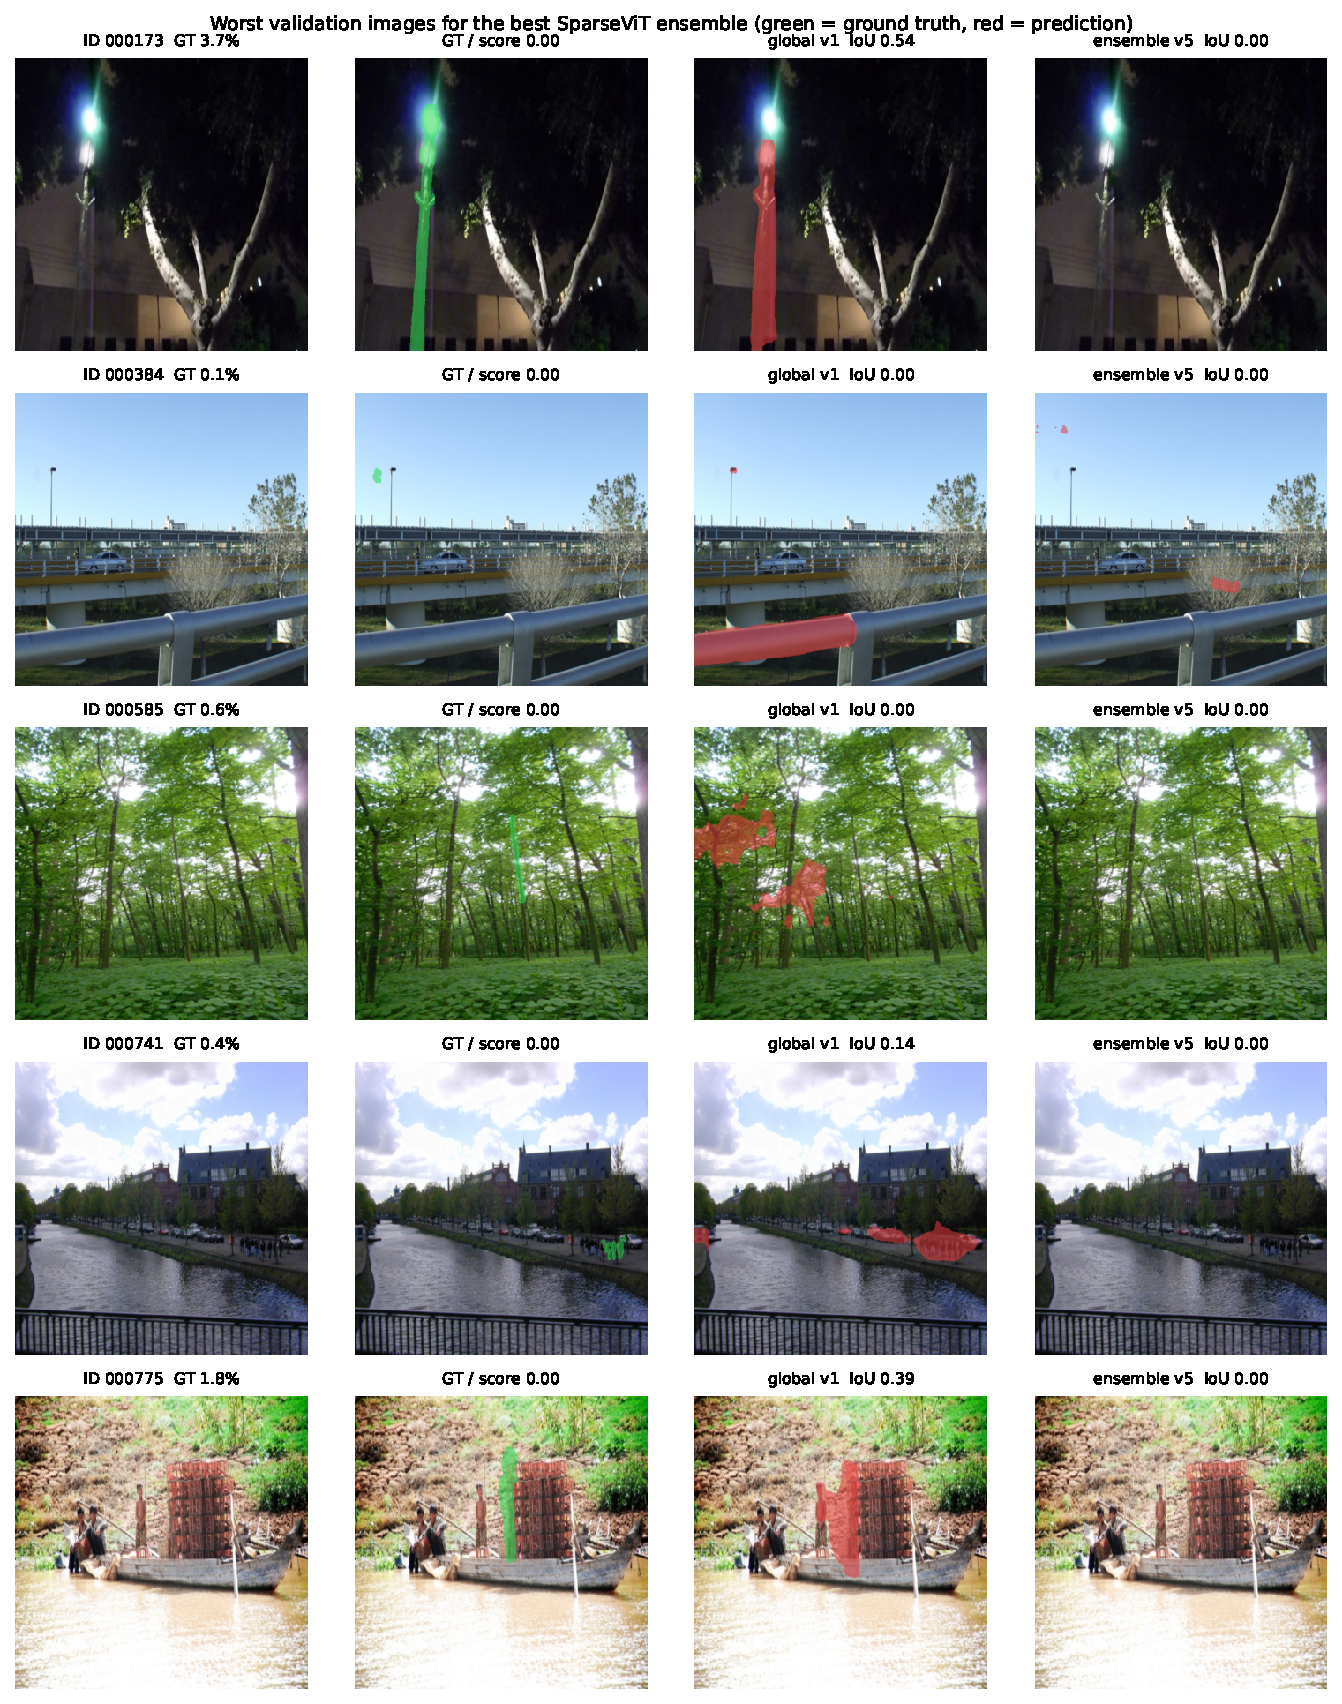
\includegraphics[width=\linewidth]{fig_val_errors}
\smallskip

\scriptsize Worst validation images: GT green, prediction red.
\column{.60\textwidth}
\scriptsize
GT has 4.22 components/image; the global model predicts 1.83 with a median size over twice as large.
\vspace{.15cm}

\begin{tabular}{lrr}
\toprule GT edited area & Images & Mean Score \\
\midrule
$0$--$0.1\%$ & 3 & 0.3115 \\
$0.1$--$1\%$ & 85 & 0.6587 \\
$1$--$5\%$ & 168 & 0.7757 \\
$>5\%$ & 244 & 0.8746 \\
\bottomrule
\end{tabular}
\vspace{.15cm}

Worst clean-validation cases:
\begin{tabular}{lrr}
\toprule ID & Score & Oracle \\
\midrule
003549 & 0.7063 & 0.803 \\
003560 & 0.7781 & 0.724 \\
004315 & 0.7793 & 0.804 \\
003501 & 0.7870 & 0.839 \\
\bottomrule
\end{tabular}
\vspace{.1cm}

For 003549, probability is 0.654 on GT pixels and 0.001 on background.
\end{columns}
\end{frame}

\begin{frame}{The current family is saturated; DINO does not help}
\begin{columns}[T]
\column{.50\textwidth}
\small
Clean-validation oracle (56 images):
\begin{tabular}{lr}
\toprule Rule & Score \\
\midrule
Teacher + hysteresis & 0.95008 \\
Hard + hysteresis & 0.93977 \\
Current fusion & 0.95314 \\
Oracle per-pixel & 0.95493 \\
\bottomrule
\end{tabular}
\vspace{.1cm}
Headroom inside this family: \textbf{0.0018}. Hysteresis sweeps, component filtering, TTA16, 640px tiles, and pseudo-label v2 all stayed at $\le 0.95314$.
\column{.48\textwidth}
\small
DINOv2-S/14 on 448 patches:
\begin{tabular}{lr}
\toprule Variant & Score \\
\midrule
Standalone DINO-HF & 0.46513 \\
Frozen DINO probe & 0.47829 \\
DINO-injected teacher & 0.90527 \\
Teacher baseline & 0.90953 \\
\bottomrule
\end{tabular}
\vspace{.1cm}
Frozen semantic tokens add no localisation signal. Stop this direction.
\end{columns}
\end{frame}

\begin{frame}{A complementary architecture: Mesorch-PT}
\small
Mesorch (AAAI'25) = DCT high-frequency CNN branch + low-frequency transformer branch, eight decoded scales and learned pixel-wise weighting. We reimplemented the paper's modules; the local encoder is standard ImageNet-1K ConvNeXt-Tiny (31.17M parameters), no author code or weights.
\vspace{.15cm}
\begin{columns}[T]
\column{.48\textwidth}\footnotesize
\begin{itemize}
\item Smoke 800/160 patches: 0.813 vs 0.37 from scratch
\item Full 20000 steps: patch-val \textbf{0.90983} (teacher 0.92052)
\item Clean-val standalone \textbf{0.94712} (teacher 0.93914)
\item Mesorch + hard, equal weights: \textbf{0.95516}
\end{itemize}
\column{.50\textwidth}\footnotesize
Same-protocol teacher+hard baseline: 0.94472. Three-way fusion with teacher adds nothing. Consensus gate reverts extreme Mesorch disagreements to the old fusion (0/56 val, 2/500 test).
\vspace{.1cm}

Kaggle: \textbf{0.94005} (ref 58928971), $+0.00981$ over previous canonical.
\end{columns}
\end{frame}

\begin{frame}{Boundary errors are ambiguous, not misaligned}
\small
\begin{columns}[T]
\column{.48\textwidth}\footnotesize
Misclassified boundary pixels have lower image gradient ($0.0454$) than correct boundaries ($0.0526$): errors lie in low-contrast, feathered edits, not at displaced strong edges.
\vspace{.1cm}

Worst-case overlays: green TP, red FP, blue FN; dominant error is missed edited pixels.
\column{.50\textwidth}\footnotesize
\begin{tabular}{lr}
\toprule Method & Clean-val Score \\
\midrule
Mesorch+hard fusion & 0.95516 \\
Gaussian $\sigma=0.5$ / $2$ & 0.95430 / 0.94351 \\
Bilateral filtering & 0.94504--0.94687 \\
Hysteresis sweep best & 0.95603 \\
Full-resolution probs & 0.95219 \\
\bottomrule
\end{tabular}
\vspace{.1cm}
Smoothing, CRF-style filters and full-resolution probabilities do not help; remaining uncertainty is intrinsic.
\end{columns}
\end{frame}

\begin{frame}{Refiner experiment: negative result}
\small
The historical checkpoint reproduces the teacher cache exactly (MAD 0), and cached masks are true GT. A width-16 U-Net refines the teacher probability from RGB, FFT/Sobel high-frequency maps, and probability edges on 9000 native patches with true labels. The refined map replaces the teacher term in the unchanged 0.4/0.6 fusion.
\vspace{.2cm}
\begin{enumerate}
\item Patch validation Score $> 0.90953$
\item Clean-validation fusion Score $> 0.953140$
\item Two-column RLE dry-run passes; submit only through GitHub Action
\item Canonical changes only after Kaggle confirms Score $> 0.93024$ (gate at that time)
\end{enumerate}
\vspace{.1cm}
\textbf{Result.} Residual refiner ties teacher on an 80-image smoke ($+10^{-5}$) but scores $0.928925 < 0.928931$ on all 500 validation images: gate fails, so no full training and no submission.

\vspace{.1cm}
\textbf{Conclusion.} The teacher/hard family was saturated; a second learned architecture delivered the confirmed gain to 0.94005. Postprocessing does not help, so further progress needs stronger or more diverse learned signals.
\end{frame}

\end{document}
